% -*- coding: utf-8; -*-
% vim: set fileencoding=utf-8 :
\documentclass[english,submission]{programming}
%% First parameter: the language is 'english'.
%% Second parameter: use 'submission' for initial submission, remove it for camera-ready (see 5.1)

\usepackage[backend=biber]{biblatex}
\addbibresource{references.bib}

\providecommand{\tightlist}{%
  \setlength{\itemsep}{0pt}\setlength{\parskip}{0pt}}

\begin{document}

\title{{[}DRAFT, please don't distribute{]} Wildcard: a tool for
modifying websites by directly manipulating data tables}
\subtitle{}% optional

\author{Geoffrey Litt}
\authorinfo{is bla bla bla}
\author{Daniel Jackson}
\authorinfo{is bla bla bla}
\affiliation{Massachusetts Institute of Technology}

\keywords{programming journal, paper formatting, submission preparation} % please provide 1--5 keywords


%%%%%%%%%%%%%%%%%%
%% These data MUST be filled for your submission. (see 5.3)
\paperdetails{
  %% perspective options are: art, sciencetheoretical, scienceempirical, engineering.
  %% Choose exactly the one that best describes this work. (see 2.1)
  perspective=art,
  %% State one or more areas, separated by a comma. (see 2.2)
  %% Please see list of areas in http://programming-journal.org/cfp/
  %% The list is open-ended, so use other areas if yours is/are not listed.
  area={Social Coding, General-purpose programming},
  %% You may choose the license for your paper (see 3.)
  %% License options include: cc-by (default), cc-by-nc
  % license=cc-by,
}
%%%%%%%%%%%%%%%%%%

%%%%%%%%%%%%%%%%%%
%% These data are provided by the editors. May be left out on submission.
%\paperdetails{
%  submitted=2016-08-10,
%  published=2016-10-11,
%  year=2016,
%  volume=1,
%  issue=1,
%  articlenumber=1,
%}
%%%%%%%%%%%%%%%%%%

%%%%%%%%%%%%%%%%%%%%%%%%%%%%%
% Please go to https://dl.acm.org/ccs/ccs.cfm and generate your Classification
% System [view CCS TeX Code] stanz and copy _all of it_ to this place.
%% From HERE
\begin{CCSXML}
<ccs2012>
<concept>
<concept_id>10002944.10011122.10003459</concept_id>
<concept_desc>General and reference~Computing standards, RFCs and guidelines</concept_desc>
<concept_significance>300</concept_significance>
</concept>
<concept>
<concept_id>10010405.10010476.10010477</concept_id>
<concept_desc>Applied computing~Publishing</concept_desc>
<concept_significance>300</concept_significance>
</concept>
</ccs2012>
\end{CCSXML}

\ccsdesc[300]{General and reference~Computing standards, RFCs and guidelines}
\ccsdesc[500]{Applied computing~Publishing}

% To HERE
%%%%%%%%%%%%%%%%%%%%%%%

\maketitle

% Please always include the abstract.
% The abstract MUST be written according to the directives stated in 
% http://programming-journal.org/submission/
% Failure to adhere to the abstract directives may result in the paper
% being returned to the authors.
\begin{abstract}
Browser extensions and user scripts can modify websites in useful
ways---ranging from blocking ads to adding entire new features to
Gmail---but many people have unique needs that aren't met by existing
extensions. Today, most of those people are stuck. They can't build
their own browser extensions without learning how to program, so they
have no choice but to accept the way the software was built. What if
things were different?

Wildcard is a platform that empowers anyone to build browser extensions
and modify websites to meet their own specific needs. Wildcard shows a
simplified view of the data in a web page as a familiar table view.
People can directly manipulate the table to sort/filter content, add
annotations, and even use spreadsheet-style formulas to pull in data
from other websites. The key idea is that a table is a powerful, simple,
and familiar paradigm for modifying a website.
\end{abstract}


\hypertarget{introduction}{%
\section{Introduction}\label{introduction}}

Todos in intro:

Do somes tuff

\begin{itemize}
\tightlist
\item
  hook with Airbnb sort
\item
  add more reasons
\item
  make this shorter
\end{itemize}

People have complaints about web apps they use, but they rarely modify
those apps to meet their needs. Why not? Some guesses:

\begin{itemize}
\tightlist
\item
  Technical skill: Most people don't know how to use Javascript and
  manipulate the DOM.
\item
  Low ROI: It takes a long time to reverse engineer a site, and it's
  usually not worth it
\end{itemize}

These seem reasonable but they might not tell the whole story.

There have been many research projects that try to address these
hurdles. For example, Chickenfoot \autocite{miller2010} allows for
people to more quickly modify sites without using Javascript or dealing
with the DOM, directly addressing both of these barriers. But, a decade
later, not many people have ended up using systems like this.

\hypertarget{why-dont-people-tweak-websites}{%
\subsubsection{Why don't people tweak
websites?}\label{why-dont-people-tweak-websites}}

I know how to do web programming, and yet I rarely modify my apps.
Sometimes it actually turns out to be pretty easy to hack on a site once
I start doing it so the ROI is actually pretty high. These reasons don't
seem to fully explain my behavior.

A disheartening explanation might be that most people just don't care
enough to make changes. This claim might be true in the current context,
but it's also important to remember that motivation is connected to
culture and to the space of possibilities provided by our tools. Most
people probably didn't want to write letters before mass literacy.

One interesting explanation is that \textbf{people can't estimate the
difficulty of a change}. It's not motivating to think about what changes
I might want when I don't know whether they would take a few minutes or
are completely impossible. For me, an engineer, this gets at the heart
of the issue. I know I could probably implement the change, but it's so
hard to estimate how long it would take (minutes? months?) that I don't
even bother trying. In general, when something seems expensive to do (or
even possibly expensive), it can discourage casual lightweight
experimentation.

So, perhaps to encourage people to casually modify software,
\textbf{apps need to provide more consistent affordances indicating what
changes are possible and easy.} Maybe if it were more obvious that
certain types of changes could be achieved in mere minutes, programmers
and non-programmers would end up modifying our software more.

\hypertarget{the-wildcard-platform}{%
\subsubsection{The Wildcard platform}\label{the-wildcard-platform}}

Wildcard adds a panel to the bottom of a web page that shows a
structured table view of some of the core data in the page. When the
user manipulates the table, the original page also gets modified. We aim
to make the mapping between the table and the page as direct and
intuitive as possible.

Todos here:

\begin{itemize}
\tightlist
\item
  a better demo is actually sorting too at this point too, to show the
  bidirectional nature
\item
  hint at future possibilities
\item
  introduce an image fallback for the PDF version
\end{itemize}

For example, in Fig.~\ref{fig:table} we open up a table view that
corresponds to search results on the Airbnb travel site.

\begin{figure}
\hypertarget{fig:table}{%
\centering
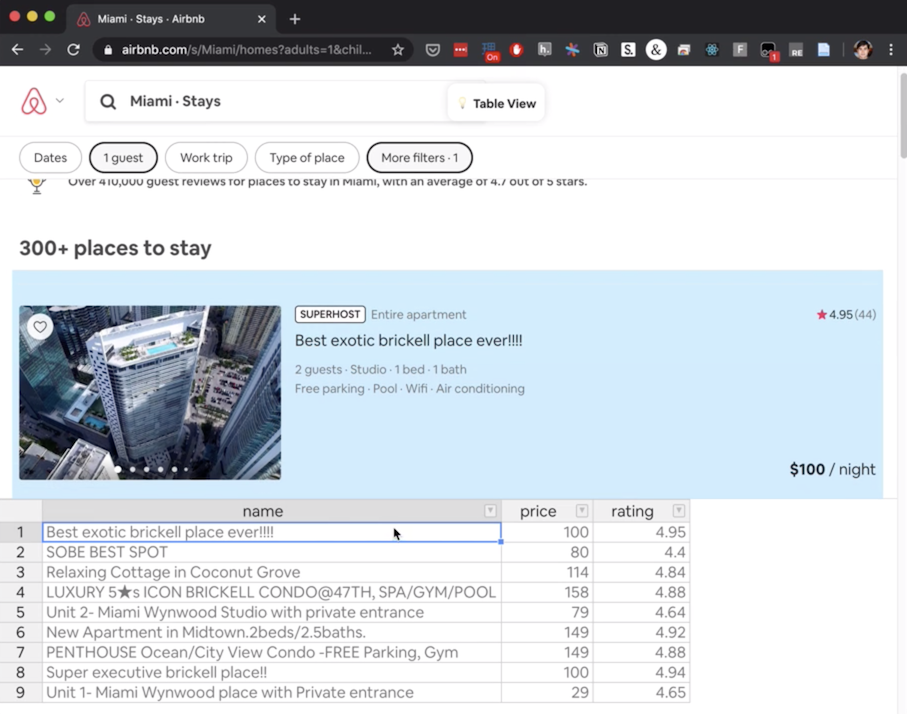
\includegraphics{media/opentable.png}
\caption{Opening a table corresponding to search results on
Airbnb}\label{fig:table}
}
\end{figure}

There's somewhat of a tension here between directness and structure.
Manipulating the original page itself might seem most ``direct.'' But
the whole problem we're dealing with is that the original web page
doesn't provide affordances for end-user modification, and there's no
consistent structure that people can learn to work with across many
sites.

\hypertarget{directness}{%
\subsubsection{Directness}\label{directness}}

The table view is perhaps one hop less ``direct,'' but in turn provides
other benefits. Because many people are already familiar with
spreadsheets, they can quickly intuit which changes are easy to make in
this system. Also, people can learn to work with the same consistent
spreadsheet view across many sites. This consistency is very
important---learning a generic tool that can be applied to many
different specific cases is very powerful, and connected to the idea of
literacy in a medium (just ask anyone who has used vim, or spreadsheets,
or a pencil and paper). Wildcard aims to balance this tension, with a
workflow that involves both the table view and the original webpage.

Wildcard is fairly general and can support many useful changes to
websites, which will be demoed later:

\begin{itemize}
\tightlist
\item
  sorting and filtering data: eg sorting shopping results
\item
  using 3rd-party APIs and performing small computations to add new
  data, in the style of ``web mashups'': eg adding walkability scores to
  hotel listings
\item
  adding private user annotations to the page: eg taking notes on
  different options
\item
  using alternate UI widgets to enter data into a page: eg using a
  personal datepicker widget with private calendar data, to enter the
  right dates for taking a flight
\end{itemize}

The overall goal is to provide generic tools that fit well with the
table paradigm and enable many specific useful changes. But it's
important to note that Wildcard doesn't aim to provide maximum coverage
all the possible ways someone might want to modify a web page. Rather,
it aims to provide a useful, simple subset of modifications, and to
provide consistent affordances so that users confidently understand
which modifications they can make.

\hypertarget{the-big-picture}{%
\subsubsection{The big picture}\label{the-big-picture}}

Eventually web apps might provide the structured data table themselves.
In the meantime, we need some sort of adapter to make this system work
with existing sites.

Wildcard provides a system for creating a wrapper on top of existing
websites. This wrapper defines how structured data can be extracted out
of the page, and also how manipulating the table should modify the page.

The most basic way of building these wrappers is for skilled programmers
to manually build and maintain them for popular sites. This approach
beats the status quo because many people, including end users, can
benefit from the generic wrapper and use it in many ways. This is
different from the current world where programmers build
use-case-specific browser extensions, and each extension has to
implement its own interactions with the low-level DOM of a page. There's
also a greater incentive for many people to collectively maintain a
wrapper if it's shared.

A more advanced way would be to make these wrappers partially or totally
automated, and enable end users to create them. This future work could
leverage existing research on wrapper induction but isn't the focus of
the current work.

Again, ultimately we hope that first-party sites would find it
beneficial and straightforward to provide a structured data view
themselves. Wildcard doesn't require sites to expose some complex
Semantic Web schema; it merely asks for a simple structured data view.

\hypertarget{demo}{%
\section{Demo}\label{demo}}

\begin{itemize}
\tightlist
\item
  Sorting search results:

  \begin{itemize}
  \tightlist
  \item
    Airbnb took away search
  \item
    once you see the tabular view, there's an obvious interaction
    available to anyone familiar with tables
  \end{itemize}
\item
  Injecting new data into the page

  \begin{itemize}
  \tightlist
  \item
    Take own custom notes, saved in the browser. Maybe shared in the
    future
  \end{itemize}
\item
  Formulas

  \begin{itemize}
  \tightlist
  \item
    Compute values to inject into the page
  \item
    TBD: styling
  \end{itemize}
\item
  Using a custom date picker
\end{itemize}

\hypertarget{design-principles}{%
\section{Design principles}\label{design-principles}}

\hypertarget{expose-generic-structure}{%
\subsection{Expose generic structure}\label{expose-generic-structure}}

\begin{itemize}
\tightlist
\item
  Consistent across all sites, can gain familiarity
\item
  Nightmare bike: users learn the structure they can exploit
\end{itemize}

\hypertarget{no-api-needed}{%
\subsection{No API needed}\label{no-api-needed}}

\begin{itemize}
\tightlist
\item
  3p-only is enough. 1p help is optional.
\item
  Can even do things the 1p didn't want to expose.
\end{itemize}

\hypertarget{in-place-toolchain}{%
\subsection{In-place toolchain}\label{in-place-toolchain}}

\begin{itemize}
\tightlist
\item
  meet the user where they are, in the page
\item
  very native to the web style (dev tools is kinda like this)
\end{itemize}

\hypertarget{decouple-ui-from-data}{%
\subsection{Decouple UI from data}\label{decouple-ui-from-data}}

\begin{itemize}
\tightlist
\item
  bring your own views of the data
\item
  bring your own widgets for data entry
\item
  instrumental interaction
\end{itemize}

\hypertarget{analysis}{%
\section{Analysis}\label{analysis}}

Cognitive dimensions?

\hypertarget{related-work}{%
\section{Related work}\label{related-work}}

\begin{itemize}
\tightlist
\item
  Instrumental interaction
\item
  Web automation
\item
  Wrapper induction
\item
  Personal data
\item
  Extension helpers
\end{itemize}

\hypertarget{future-work-open-questions}{%
\section{Future work / Open
Questions}\label{future-work-open-questions}}

\begin{itemize}
\tightlist
\item
  How far does functionality go?

  \begin{itemize}
  \tightlist
  \item
    workflows? triggers?
  \item
    what can and can't be done?

    \begin{itemize}
    \tightlist
    \item
    \end{itemize}
  \end{itemize}
\item
  automated wrappers?

  \begin{itemize}
  \tightlist
  \item
    lean on existing tech
  \end{itemize}
\item
  usability studies
\end{itemize}

\hypertarget{conclusions}{%
\section{Conclusions}\label{conclusions}}

\hypertarget{todos}{%
\section{Todos}\label{todos}}

\begin{itemize}
\tightlist
\item
  remove bold text for the proceedings version
\end{itemize}

\acks
\printbibliography

\end{document}

% Local Variables:
% TeX-engine: luatex
% End:
